% CREATED BY DAVID FRISK, 2016
\chapter{Theory}

	% vi måste bestämma oss för vad vi kallar algoritmen. nu har vi 2
	% konkurrerande termer
	The algorithm in question that we designed a custom GPU for is called
	Sphere Tracing\cite{Hart1996}. The name comes from the technique where it uses spheres to
	incrementally advance a ray in 3D space. The method of advancing rays
	incrementally is called Ray Marching and is a particular subset of ray
	tracing.\cite{Whitted1980} Ray Tracing, then, is a way of wholly or
	partially rendering the world through rays, cast from the eye of the
	observer into the scene. Sphere Tracing has been around since at least as
	early as the late eighties and Ray Tracing as early as the
	sixties\cite{Hart1989,Appel1968}. Ray Tracing has traditionally been a 
	more computationally intensive method compared to polygon
	rendering\cite{Wylie1967} and thus it has generally seen more use in movie  
	production rather than in real-time applications.\cite{ref_needed?} 
	
	The advent of per pixel programmable hardware in graphics cards made it 
	possible to implement real time graphics rendering based on ray	marching, 
	albeit only using relatively simple geometry. This raises the question of 
	whether this rendering method could be competitive for real time graphics, 
	if hardware that was specifically designed for it was available.
	
		
	\section{Sphere Tracing} 

		\begin{wrapfigure}{r}{0.48\textwidth}
			\begin{flushright}
				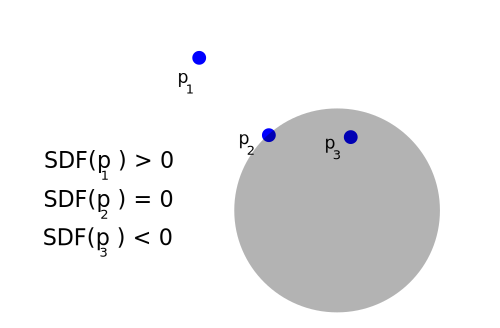
\includegraphics[width=0.9\linewidth]{figure/SDF} 
			\end{flushright}
			\caption{ Signed Distance Function of a sphere, sampled at three points}
			\vspace{40pt}
		\end{wrapfigure}
		
		The sphere tracing algorithm is based on the concept of Signed Distance Functions (SDF).
		$$\text{SDF}:\mathbb{R}^{3}\mapsto\mathbb{R}$$ 
		The "distance" is the distance between a point and the closest point on the implicit surface $\text{SDF}^{-1}(0)$. 
		%vad betyder detta och vad är det för funktion? borde vi inte ge ett exempel på en sådan funktion?
		The "signed" part refers to the
		distance being negated when measured on the other side of the
		surface. If we define a ray $$r(s) = \vec{d} \cdot s + \vec{o}$$
		where $\vec{d}$ is the direction of the ray and $\vec{o}$ the 
		origin, then $$\text{SDF}\circ r(s) = 0$$ means that the ray
		intersects a surface at exactly the distance $s$ from its origin.
		\emph{ Sampling every SDF in a given scene and returning the smallest 
			value yields a function known as a distance field.
		}

		\bigskip
		\noindent Finding the surface can be done by iterating point by point from the
		origin along the ray like below: $$p_{i+1} = p_i + \vec{d}\cdot
		\text{SDF}(p_i)$$ This is repeated until $\text{SDF}(p_i) \leq
		\varepsilon$ for a given precision limit $\varepsilon$.
		$\text{SDF}(p_i)$ is the furthest possible march distance the ray can 
		march while still being sure not too overshoot any potential surfaces.  
		The direction of the closest surface point is never known, thus 
		$\text{SDF}(p_i)$ can be interpreted as a spherical bound, giving the 
		algorithm it's name. This Ray Marching is then performed for each pixel 
		of the screen, reversely simulating the light rays entering the lens of 
		an eye or camera.
			
			\subsection{Reflections and refractions}
		
				Once a point on a surface for a given pixel has been located
				new multiple rays can then march further to determine
				reflections, towards the scene's sources of light determining
				light and shadows, or through the object with an angle,
				simulating refractions. A lot of these depend on the surface
				normal which can be calculated by normalizing the approximate
				gradient of $\text{SDF}(p)$. 
		
			\subsection{Materials}
				Coloring a certain ray in a scene is based on the material ID
				assigned to the first object that the ray intersects. The color
				can then be either calculated by a material formula or be 
				derived from a texture lookup. True 3D materials can be done by
				texturing but this generally needs a large data set and thus a 
				formula is mostly preferred where three dimensional materials 
				are employed. 2D texturing can be done by projecting points from
				a flat image onto a simple geometric shape  which is more or less 
				enveloping the object in question. This is called texture-mapping 
				and commonly uses simple shapes like planes, cubes, spheres and 
				cylinders. 
				
				Light can be calculated by taking the angle of incidence between
				the previously mentioned surface normal and the direction of one 
				or more predefined light sources. Shadows can be calculated by 
				ray marching from the intersection point to the lights and 
				applying shadowing if the path traversed was intersected by any
				object in the scene. 
				
				Light and shadow values are then blended with the material color,
				based on parameters from the material ID, to form the final 
				output pixel color.
						
				%%\footnotetext{Or along the normal of the point.}
		
